\cleardoublepage
\begin{minipage}{0.95\linewidth}

\part{Implémentations et Expérimentations}
\vspace{15mm} % l'espacement souhaité
\parttoc 
\end{minipage}
\newpage
\thispagestyle{empty}
\vspace*{\stretch{1}}
\begin{center}
  \begin{minipage}{\textwidth}
    \hrule
    \vspace{0.5cm}
    {\it  La dernière partie de cette thèse est consacrée à la
      présentation des résultats des expérimentations que nous avons
      conduites pour valider les méthodes présentées dans les
      chapitres précédents. Nous commençons, dans un premier temps,
      par présenter les instances sur lesquelles ces expérimentations
      ont été menées ainsi que les algorithmes de prétraitement
      utilisés. 

      La suite de cette partie est ensuite consacrée à la présentation
      des résultats des méthodes décrites dans le
      chapitre~\ref{sec:PLNE_CECSP} et issues de la programmation linéaire
      mixte. Le modèle indexé par le temps pour le \CECSP~est comparé
      à ce même modèle auquel on a ajouté les inégalités déduites du
      raisonnement énergétique et présentées dans le
      paragraphe~\ref{sec:ER_TI}. Pour les modèles à événements, nous
      commençons par détailler l'algorithme utilisé pour séparer les
      inégalités de non-préemption (voir
      paragraphe~\ref{sec:nonPreem}). Les modèles sont ensuite comparés
      entre eux et l'ajout des inégalités et coupes décrites dans le
      paragraphe~\ref{sec:amelioration_OO} au modèle On/Off dans le cas du
      \CECSP~et du \RCPSP~est discuté. La dernière partie du paragraphe
      traitant de la programmation linéaire est consacrée à la comparaison
      des trois modèles.

      Le dernier paragraphe concerne les résultats des méthodes issues de
      la programmation par contraintes présentées dans le
      chapitre~\ref{sec:PPC_CECSP}. Dans un premier temps, nous
      décrivons le cadre dans lequel ces expérimentations ont été
      conduites: les algorithmes de propagation détaillés dans ce manuscrit
      sont inclus dans une méthode arborescente hybride. Une fois le cadre
      des expérimentations posé, nous comparons les trois méthodes permettant
      de calculer les intervalles d'intérêt du raisonnement
      énergétique. Enfin, la suite de cette partie détaille les résultats de
      cette méthode arborescente avec les différents algorithmes de
      propagation. 

    Dû à la difficulté du \CECSP, les expérimentations présentées
    dans cette partie ont majoritairement été conduites sur des
    instances dans lesquelles les activités ont des fonctions de
    rendement affines. Quelques résultats sur des instances de petite
    taille avec des fonctions de rendement concaves et affines par
    morceaux sont présentés à la fin de cette partie.}
    \vspace{0.5cm}
    \hrule
  \end{minipage}
\end{center}
\vspace*{\stretch{1}}

\chapter{Implémentations et Expérimentations}
\label{sec:expe}

Dans ce chapitre, consacré à la présentation des résultats
expérimentaux, nous allons, dans un premier temps, décrire les
jeux d'instances utilisés ainsi que certaines méthodes de
prétraitement qui sont appliquées à ces instances avant leur
résolution. 

Le paragraphe suivant sera quant à lui dédié aux résultats de la
programmation linéaire mixte et en nombres entiers. Nous présenterons
les performances des différents modèles présentés dans le
chapitre~\ref{sec:PLNE_CECSP} ainsi que l'impact des améliorations
proposées dans le paragraphe~\ref{sec:amelioration_modele} de ce même
chapitre. 

Le dernier paragraphe sera consacré à la présentation des performances
de la programmation par contraintes où les performances des
algorithmes de filtrage présentés dans le chapitre~\ref{sec:PPC_CECSP}
seront comparées. 

Tous les tests ont été effectués avec un processeur Intel Core i7-4770
de 3.40GHz, 8 GB de RAM, tournant sous le système d’exploitation
Ubuntu 12.04 à 64-bits. Toutes les méthodes présentées ont été codées
en C++. Les programmes linéaires mixtes sont résolus avec le solveur
commercial ILOG-Cplex version 12.6.

%TODO : fonction LPM et résultats time index RCPSP avc RE?
\section{Génération des instances et pré-traitement}

Ce paragraphe présente, dans un premier temps, la méthode utilisée
pour générer des ensembles d'instances de test pour le \CECSP. Nous
détaillons ensuite les jeux d'instances du \RCPSP sur lesquelles nous
avons évalué l'impact des améliorations proposées pour les modèles à
événements. Nous présenterons aussi une méthode de calcul des fenêtres
de temps pour le \RCPSP, appliqué sur les instances comme
pré-traitement à leur résolution.

\subsection{Instances du \CECSP}
\label{sec:instance_CECSP}
Les instances utilisées dans le cadre du \CECSP sont regroupées en
quatre familles selon les caractéristiques de leurs fonctions de
rendements et de l'énergie que les activités requièrent. Dans un
premier temps, les instances sont générées selon un modèle commun,
puis plusieurs types de modifications spécifiques sont appliquées sur
celles-ci afin de les séparées en différentes familles. 

Tout d'abord, cinq instances de $10$ et $60$ activités ainsi que dix
instances de respectivement $20$, $25$ et $30$ activités sont
générées. Pour toutes ces instances, la disponibilité de la ressource
est fixée à $R=10$ et les autres paramètres du problème sont générés
de façon aléatoire selon une loi uniforme et dans les intervalles
suivants:
\begin{itemize}
\item $W_i \in [1 , \frac{5}{4} * R]$,
\item $\bmin \in [0, \frac{1}{4} * W_i]$,
\item $\bmax \in [\bmin , 2 * \bmin {]}$,
\item $\ES \in [0,\frac{1}{2}*n]$ et
\item $\LE \in [ \EE, \EE + n ]$ avec $\EE = \ES +
\frac{W_i}{f_i(\bmax)}$.
\end{itemize}

Une première famille d'instance, appelée Famille 4, est construit en
utilisant comme fonction de rendement la fonction identité pour toutes
les activités, i.e. $\forall i \in \A,\ f_i(b_i(t))= b_i(t)$. Ensuite,
des fonctions de rendement affines sont générées aléatoirement pour
chaque activité. Pour cela, nous générons, pour chaque activité $i \in
\A$, les paramètres $a_i$ et $c_i$ de la fonctions $f_i$ suivant une
loi uniforme et telle que:
\begin{itemize}
\item $a_i \in [1,10]$ et
\item $c_i \in [1,10]$.
\end{itemize} La valeur de $W_i$ est ensuite modifiée à l'aide de ces
fonctions $f_i$. Les trois autres familles d'instances sont classées
suivant cette modification. Pour la première famille, appelée Famille
1, $W_i$ est généré aléatoirement, selon une loi uniforme, dans
l'intervalle $[0,f_i(W_i)]$ et pour la Famille 2 dans l'intervalle
$[f_i(W_i)/2, f_i(W_i)]$. Enfin, pour la Famille 3, la valeur
$f_i(W_i)$ est affectée $W_i$. 

Nous avons donc défini quatre familles d'instances pour le \CECSP. Ces
instances serviront à calculer les performances relatives des méthodes
présentées dans les chapitres précédents de ce manuscrit. 

Dans le prochain paragraphe, nous présentons les instances utilisées
pour évaluer les performances des améliorations des modèles du
\RCPSP~ainsi qu'une méthode de calcul des fenêtres de temps.
  
\subsection{Instances et pré-calcul des fenêtres de temps pour le
  \RCPSP}
\label{sec:instances_RCPSP}
\subsubsection{Génération des instances}
Les instances utilisées sont les instances définies par
Kone~\cite{theseOumar} pour évaluer la performances des modèles à
événements par rapport aux modèles indexés par le temps. Ces instances
sont générées à partir des instances à $30$ activités de la
PSPLIB~\cite{PSPLIB}. Ces instances, au nombre de $480$, sont des
instances à $4$ ressources renouvelables et avec des activités ayant
une durée aléatoire comprise entre $1$ et $10$ unités de temps. Ces
durée étant relativement courtes, les modèles indexés par le temps
sont particulièrement efficaces sur ces dernières (voir
paragraphe~\ref{sec:motiv_event_RCPSP}). L'auteur de~\cite{theseOumar}
a donc modifié ces instances afin d'allonger la durée des
activités. En effet, dans certaines applications pratiques (notamment
dans le domaine pharmaceutique ou de la pétrochimie), il arrive que
les activités aient des durées relativement longues.

Les instances de Kone sont crées selon le principe suivant: 
\begin{enumerate}
\item les $15$ premières activités non-fictives de l’instance sont
  sélectionnées (les autres activités ainsi que les contraintes de
  précédence qui leur sont adjacentes sont laissées de côté).
\item parmi les activités sélectionnées, celles sans prédécesseurs
  sont connectées à l’activité 0 et celles sans successeurs à l’activité
  $16$.
\item  $7$ activités parmi les $15$ sélectionnées sont ensuite
  choisies de façon aléatoire et leur durée est multipliée par un
  coefficient $25+b$, où $b$ est un nombre aléatoire généré entre $0$
  et  $1$.

  Les durées obtenues sont ensuite arrondies au nombre entier le plus
  proche. 
\end{enumerate}
$480$ instances de taille plus réduite sont obtenues ($n=15$), mais
avec des durées opératoires plus grandes, allant ainsi de $1$ à
approximativement $250$ unités de temps. 

\subsubsection{Calcul des fenêtres de temps}

Afin d'améliorer les performances des modèles pour le \RCPSP, nous
calculons par prétraitement, pour chaque activité, les fenêtres de
temps $[\ES,\LS{]}$ et $[\EE,\LE{]}$ dans lesquelles elle peut
respectivement commencer et finir. Pour calculer ces fenêtres de
temps, rappelons que, si chaque arc $(i,j)$ du graphe des précédences
$G$ est pondéré par $p_i$, la date de début au plus tôt de $i$, $\ES$
peut prendre la valeur du plus long chemin entre l'activité $0$ et
l'activité $i$ et la date de début au plus tard $\LS$ est égale à
$\ES[n+1]$, la date de début au plus tôt de l'activité terminale
$n+1$, moins la valeur du plus long chemin entre $i$ et $n+1$.

Notons que la date de fin au plus tard de l'activité fictive $n+1$
correspondant à une borne supérieure sur la date de fin du projet peut
être calculée au moyen d'une heuristique. L'heuristique utilisée pour
calculer cette valeur ici est la méthode d'ordonnancement parallèle
avec comme règle de priorité la plus petite date de fin au plus tard
des activités~\cite{heur_RCPSP}. 

En plus des calculs décrits ci-dessus, nous utilisons d'autres
techniques de déductions basées sur la propagation de contraintes. En
particulier, nous utilisons des techniques décrites dans la thèse de
Demassey~\cite{these_Sophie}. Parmi celles utilisées, nous trouvons
les techniques de sélection immédiate, Edge-Finding sur les cliques de
disjonction et de triplets symétriques. Ces techniques n'étant pas
détaillées ici, à l'exception du Edge-Finding au
paragraphe~\ref{sec:nrj_CUSP}, nous renvoyons le lecteur au chapitre 2
de~\cite{these_Sophie} pour une description de ces techniques.

\section{Performances de la Programmation Linéaire Mixte}
\label{sec:expe_PLNE}
Dans ce paragraphe, nous détaillons les résultats expérimentaux
obtenus par les modèles présentés dans le
chapitre~\ref{sec:PLNE_CECSP} et l'influence des techniques de
renforcement présentées dans ce même chapitre. Nous commençons, dans
un premier temps, par présenter les résultats obtenus pour le modèle
indexé par le temps puis nous détaillerons les résultats des modèles à événement.

\subsection{Modèles indexés par le temps}
Dans ce paragraphe, nous décrivons les performances du modèle indexé
par le temps pour le \CECSP. Les expérimentations ont été conduites
sur les quatre familles d'instances présentées dans le
paragraphe~\ref{sec:instance_CECSP} et avec une limite de temps de 100
secondes. Le modèle, avec pour objectif la minimisation de la
consommation totale de ressource, est dans un premier temps utilisé
pour résoudre les instances. Dans un second temps, nous ajoutons les
inégalités issues du raisonnement énergétiques décrites dans le
paragraphe~\ref{sec:ER_TI}. Ces inégalités sont seulement ajoutées au
n\oe ud racine de l'arbre de recherche. En effet, dû à leur grand
nombre ($5*|\I|*n$, avec $\I$ l'ensemble des intervalles d'intérêt du
raisonnement énergétique) , il est difficile, sans algorithme de
séparation, de les inclure dynamiquement pendant la recherche. Le
tableau~\ref{tab:TI_CECSP} présente ces résultats.

Dans ce tableau, nous avons comparé la qualité et le temps d'obtention
des premières solutions pour chaque famille d'instances et pour les
cas avec et sans coupes énergétiques. La qualité de la solution est
mesurée de la manière suivante: 
\[
  \text{gap}=100*\frac{|\text{Objectif final} - \text{Objectif } 1^{ère} \text{  Sol}|}{\text{Objectif final}}
\]
Nous avons aussi comparé le temps nécessaire à l'obtention de la
solution optimale (100 secondes si la solution trouvée n'est pas
optimale), la qualité de la solution, le nombre d'instances résolues
et le nombre d'entre elles résolues à l'optimum.

\begin{table}[!htb]
  \begin{center}\small
    \begin{tabularx}{\linewidth}{|Y|YY|YYYY|YY|YYYY|}
      \hline
      \multirow{2}{*}{\#act.} & \multicolumn{2}{c|}{$1^{ère}$ sol.}&
      \multicolumn{4}{c|}{sol. finale} & \multicolumn{2}{c|}{$1^{ère}$ 
        sol.}&
      \multicolumn{4}{c|}{sol. finale} \\ 
      \cline{2-13} 
                               & tps(s) & gap & tps & gap  &  \%opt.&\%solv.&
                                                                 tps
                                                                 & gap
                                                                 &
                                                                 tps
                                                                 & gap
                                                                 &
                                                                 \%opt. &\%solv.  \\ 
      \hline
      \multicolumn{7}{|l|}{Famille 1} & \multicolumn{6}{|l|}{Famille 2}\\
      \hline
      \multicolumn{7}{|r|}{sans coupes énergétiques} & \multicolumn{6}{|r|}{sans coupes énergétiques}\\
      \hline  
      $10 $&$ 0,058 $&$ 38 $&$ 45 $&$ 2,9$ &$ 60 $&$ 100$ &$ 0,075 $&$ 24 $&$ 100 $&$ 5,6$ &$ 0 $&$ 100$ \\ 
      $20 $&$ 0,25 $&$ 17 $&$ 100 $&$ 8,4$ &$ 0 $&$ 100$ & $ 0,37 $&$ 8,8 $&$ 100 $&$ 6,5$ &$ 0 $&$ 100$\\ 
      $25 $&$ 0,88 $&$ 21 $&$ 100 $&$ 9,4$ &$ 0 $&$ 100$ &$ 2 $&$ 12 $&$ 100 $&$ 5,8$ &$ 0 $&$ 100$ \\ 
      $30 $&$ 1,3 $&$ 35 $&$ 100 $&$ 10$ &$ 0 $&$ 100$&$ 3,1 $&$ 14 $&$ 100 $&$ 6,3$ &$ 0 $&$ 100$  \\ 
      \hline 
      \multicolumn{7}{|r|}{avec coupes énergétiques à la racine} &  \multicolumn{6}{|r|}{avec coupes énergétiques à la racine}\\
      \hline
      $10 $&$ 0,064 $&$ 3,4 $&$ 60 $&$ 2,6$ &$ 40 $&$ 100$ &$ 0,074 $&$ 9 $&$ 100 $&$ 4,1$ &$ 0 $&$ 100$\\ 
      $20 $&$ 0,31 $&$ 18 $&$ 100 $&$ 8,7$ &$ 0 $&$ 100$& $ 0,65 $&$ 9,4 $&$ 100 $&$ 6,2$ &$ 0 $&$ 100$  \\ 
      $25 $&$ 0,63 $&$ 17 $&$ 100 $&$ 9,6$ &$ 0 $&$ 100$ &$ 1,9 $&$ 12 $&$ 100 $&$ 6$ &$ 0 $&$ 100$\\ 
      $30 $&$ 1,6 $&$ 18 $&$ 100 $&$ 10$ &$ 0 $&$ 100$ &$ 5,8 $&$ 11 $&$ 100 $&$ 6,3$ &$ 0 $&$ 100$ \\ 
      \hline   
      \multicolumn{7}{|l|}{Famille 3} &  \multicolumn{6}{|l|}{Famille 4}\\
      \hline
      \multicolumn{7}{|r|}{sans coupes énergétiques}&  \multicolumn{6}{|r|}{sans coupes énergétiques}\\
      \hline  
    $10 $&$ 0,064 $&$ 4,1 $&$ 64 $&$ 1,8$ &$ 40 $&$ 100$ &$ 0,037 $&$ 0 $&$ 0,037 $&$ 0$ &$ 100 $&$ 100$\\ 
$20 $&$ 2,8 $&$ 6,8 $&$ 100 $&$ 3,9$ &$ 0 $&$ 100$ &$ 0,61 $&$ 0,72 $&$ 0,63 $&$ 0$ &$ 100 $&$ 100$\\ 
$25 $&$ 17 $&$ 4,5 $&$ 100 $&$ 4,5$ &$ 0 $&$ 100$ &$ 1,5 $&$ 0,31 $&$ 1,5 $&$ 0$ &$ 100 $&$ 100$\\ 
$30 $&$ 24 $&$ 6,4 $&$ 100 $&$ 4,1$ &$ 0 $&$ 80$ &$ 4,8 $&$ 0,07 $&$ 15 $&$ 0$ &$ 89 $&$ 89$ \\ 
      \hline 
      \multicolumn{7}{|r|}{avec coupes énergétiques à la racine} & \multicolumn{6}{|r|}{avec coupes énergétiques à la racine}\\
      \hline
$10 $&$ 0,063 $&$ 3,4 $&$ 80 $&$ 1,8$ &$ 20 $&$ 100$&$ 0,045 $&$ 1,1 $&$ 0,046 $&$ 0$ &$ 100 $&$ 100$  \\ 
$20 $&$ 2,5 $&$ 6,7 $&$ 100 $&$ 3,8$ &$ 0 $&$ 100$ &$ 0,56 $&$ 0,64 $&$ 0,71 $&$ 0$ &$ 100 $&$ 100$  \\ 
$25 $&$ 18 $&$ 5,8 $&$ 100 $&$ 4,4$ &$ 0 $&$ 100$ &$ 2,6 $&$ 0,072 $&$ 2,9 $&$ 0$ &$ 100 $&$ 100$ \\ 
$30 $&$ 24 $&$ 7,6 $&$ 100 $&$ 4,2$ &$ 0 $&$ 70$ &$ 6,4 $&$ 0 $&$ 6,4 $&$ 0$ &$ 100 $&$ 100$\\ 
      \hline   
    \end{tabularx}
  \end{center}
  \caption{Résultats du PLNE indexé par le temps du \CECSP~avec et
    sans coupes énergétiques.} 
  \label{tab:TI_CECSP}
\end{table}

Les résultats présentés dans le tableau~\ref{tab:TI_CECSP} montrent
que, dans la majorité des cas, le modèle avec les coupes énergétiques
obtient une première solution de meilleure qualité que celle obtenue
sans ces coupes. De plus, le temps de calcul de cette première
solution, bien que légèrement plus élevé dans le cas des coupés
énergétiques, est du même ordre de grandeur dans les deux cas.

Cependant, sauf dans le cas des instances à 30 activités de la Famille
4 où l'ajout des coupes permet un gain en termes de performances, les
coupes énergétiques ne produisent pas de gain significatif, ni en
termes de qualité de solution, ni en termes de temps de résolution. 

Malgré tout, les performances relatives des coupes énergétiques pour
le calcul des premières solutions pousse à poursuivre cette
investigation. La mise en place en place d'un algorithme de séparation
permettant de trouver les meilleures coupes à ajouter à chaque n\oe ud
de l'arbre de recherche devient donc une direction de recherche
encourageante dans un futur proche. 

\subsection{Modèles à événements}

Ce paragraphe, dédié à la présentation des résultats obtenus pour les
modèles à événements, commence par présenter l'algorithme de
séparation qui sera utilisé dans le modèle On/Off pour séparer les
inégalités de non-préemption. Cet algorithme a été conçu en
collaboration avec Tam{\'a}s Kis. Nous présenterons ensuite les
différents résultats obtenus pour les modèles Start/End et On/Off.

\subsubsection{Algorithme de séparation pour les inégalités de non
  préemption} 

L'idée principale de la procédure de séparation pour les inégalités de
non préemption (voir paragraphe~\ref{sec:nonPreem} est que, pour
chaque activité $i$, trouver la coupe à ajouter au modèle est
équivalent à trouver un plus long chemin dans un certain graphe. Ce
graphe orienté et acyclique est défini de la manière suivante:
\begin{itemize}
\item à chaque événement de l'ensemble $\E^*$=$\E \setminus\{2n\}$,
i.e. $\{1,\dots,2n-1\}$, on fait correspondre un sommet;
\item on ajoute au graphe un source et un puits, indexés
respectivement par $0$ et $2n$. Le graphe est donc composé de $2n+1$
sommets.
\item L'ensemble des arcs est divisé en trois catégories:
  \begin{itemize}
  \item[(i)] les {\it arcs de départ} relient le sommet source $0$ à
chaque sommet $u \in \{1,\dots,2n-3\}$;
  \item[(ii)] les {\it arcs intermédiaires} relient les sommets $u \in
\{1,\dots, 2n-3\}$ aux sommets $v \in \{u+2,\dots,2n-1\}$ et
  \item[(iii)] les {\it arcs terminaux} relient les sommets $u \in
\{3,\dots,2n-1\}$ au sommet puits $2n$;
  \end{itemize}
\end{itemize}

De plus, un coût $cost(u,v)$ est associé à chaque arc $(u,v)$
composant le graphe. Le coût d'un arc de départ est $0$, celui d'un
arc intermédiaire $(u,v)$ est $cost(u,v)= \overline{z}_{i,u} - \min\{
\overline{z}_{i,\ell}\ :\ \ell= u+1,\dots, v-1\}$ et celui d'un arc
terminal $(u,2n)$ est $\overline{z}_{i,u}$, avec $\overline{z}_{i,u}$
la valeur de la variable correspondante. La construction de ce graphe
est illustrée dans l'exemple~\ref{ex:algo_sep}.

\begin{ex}
\label{ex:algo_sep}
Considérons une instance à quatre activités. Le nombre d'événements
$|\E|$ est égal à $8$. Considérons, par exemple, l'activité $1$. Si
nous appliquons la transformation décrite ci-dessus, nous obtenons le
graphe à $9$ sommets et $30$ arcs décrits par la
figure~\ref{fig:algo_sep}. Sur ce graphe, seuls les coûts des arcs
terminaux et des arcs intermédiaires sortant du sommet $2$ sont
représentés. 
\begin{figure}[!htb]
  \centering
  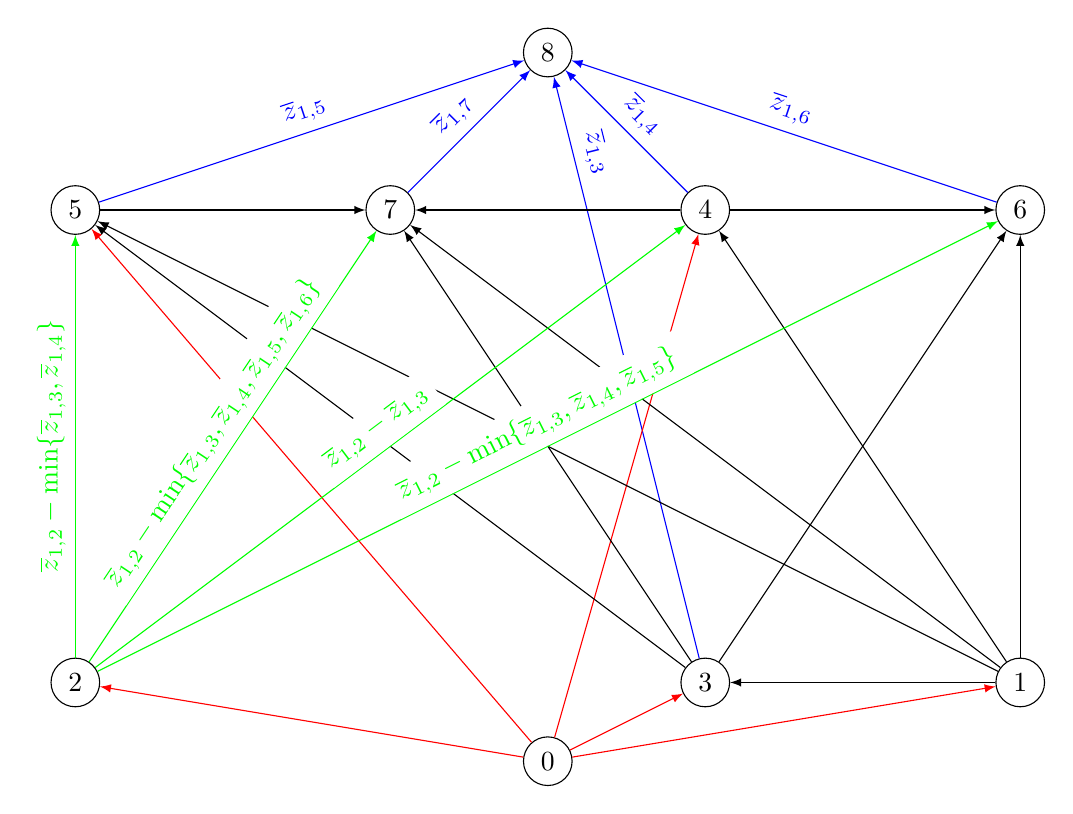
\begin{tikzpicture}
    [  every node/.style={},%
    dot/.style={circle,fill=black,minimum size=4pt,inner sep=0pt,%
      outer sep=-1pt},
    cross/.style={path picture={ 
        \draw
        (path picture bounding box.south east) -- (path picture
        bounding box.north west) (path picture bounding box.south
        west) -- (path picture bounding box.north east); 
      }}]
    \tikzstyle{sommet}=[draw,circle,minimum width=0.5cm]
    \node[sommet] (O) at (0,0) {$0$};
    \node[sommet] (U) at (6,1) {$1$}; 
    \node[sommet] (D) at (-6,1) {$2$}; 
    \node[sommet] (T) at (2,1) {$3$}; 
    \node[sommet] (Q) at (2,7) {$4$}; 
    \node[sommet] (C) at (-6,7) {$5$}; 
    \node[sommet] (Si) at (6,7) {$6$}; 
    \node[sommet] (Se) at (-2,7) {$7$};
    \node[sommet] (H) at (0,9) {$8$};
    
    \draw[->,>=latex,blue] (T) --  node[pos= 0.86,sloped, above] {$
      \overline{z}_{1,3}$} (H) ;
    \draw[->,>=latex,blue] (Q) -- node[sloped,above] {$
      \overline{z}_{1,4}$} (H) ; 
    \draw[->,>=latex,blue] (C) --  node[sloped,above] {$
      \overline{z}_{1,5}$}(H) ; 
    \draw[->,>=latex,blue] (Si) -- node[sloped,above]
    {$ \overline{z}_{1,6}$} (H)  ;
    \draw[->,>=latex,blue] (Se)  -- node[sloped,above] {$
      \overline{z}_{1,7}$} (H) ;
    
    \draw[->,>=latex,red] (O) -- (U);
    \draw[->,>=latex,red] (O) -- (D);
    \draw[->,>=latex,red] (O) -- (T);
    \draw[->,>=latex,red] (O) -- (Q);
    \draw[->,>=latex,red] (O) -- (C);
    
    \draw[->,>=latex] (U) -- (T) ;
    \draw[->,>=latex] (U) -- (Q) ;
    \draw[->,>=latex] (U) -- (C) ;
    \draw[->,>=latex] (U) -- (Si) ;
    \draw[->,>=latex] (U) -- (Se) ;
    
    \draw[->,>=latex] (T) -- (C) ;
    \draw[->,>=latex] (T) -- (Si) ;
    \draw[->,>=latex] (T) -- (Se) ;
    
    \draw[->,>=latex] (Q) -- (Si) ;
    \draw[->,>=latex] (Q) -- (Se) ;
    
    \draw[->,>=latex] (C) -- (Se) ;
    
    \draw[->,>=latex,green] (D) --node[fill=white,sloped,above]
    {$ \overline{z}_{1,2} - \overline{z}_{1,3}$} (Q) ;
    \draw[->,>=latex,green] (D) -- node[fill=white,sloped,above]
    {$ \overline{z}_{1,2} -
      \min\{\overline{z}_{1,3},\overline{z}_{1,4}\}$}(C) ; 
    \draw[->,>=latex,green] (D) -- node[fill=white,sloped,above]
    {$ \overline{z}_{1,2}-
      \min\{\overline{z}_{1,3},\overline{z}_{1,4},\overline{z}_{1,5}\}$}(Si) 
    ; 
    \draw[->,>=latex,green] (D) -- node[fill=white,sloped,above]
    {$
      \overline{z}_{1,2}-\min\{\overline{z}_{1,3},\overline{z}_{1,4},\overline{z}_{1,5},\overline{z}_{1,6}\}$}(Se)
    ; 
    
  \end{tikzpicture}
  \caption{Création du graphe de l'algorithme de séparation pour les
      inégalités de non préemption}
    \label{fig:algo_sep}
  \end{figure}
\end{ex}

Pour séparer un vecteur $\overline{z}_i \in \mathbb{R}^{\E^*}$, nous
calculons un plus long chemin dans le graphe à l'aide de la
programmation dynamique. Pour cela, nous calculons, pour chaque $v \in
\{1,\dots,2n-1\}$, la valeur  du plus long chemin jusqu'à ce somment
$F(v)$ de la manière suivante:
\begin{equation}
  F(v) = \max\{ F(u) + cost (u,v) \ : \ u=1,\dots,v-2 \}
\end{equation}
avec $F(1)=F(2)=0$. 

Puis, on ajoute à ce plus long chemin, la valeur de l'arc servant à
rejoindre le puits. Cela revient à ajouter $\overline{z}_{i,v}$ à
chaque $F(v)$. Si cette valeur est supérieure à celle du
plus long chemin trouvé jusqu'à maintenant, nous remplaçons le plus
long chemin et sa valeur par le nouveau chemin trouvé.

\begin{ex}
Considérons le vecteur $\overline{z}_1$ suivant: $(0,2\ ;\ 0\ ;\
0,4\ ;\ 0,6\ ;\ 0,6\ ;\ 0\ ;\ 1\ ;\ 0,2)$.

Nous avons $F(1)=F(2)=0$. En effet, l'inégalité devant comporter au moins
trois éléments, $F(1)$ et $F(2)$ ne pourront conduire à une telle
inégalité. La longueur du plus long chemin est initialisée à $0$ et
correspond au chemin vide. De plus,nous avons: 
\begin{itemize}
\item $F(3) =  F(1) + cost (1,3) = F(1) + \overline{z}_{1,1} -
  \overline{z}_{1,2} = 0 + 0,2 - 0= 0,2 $. 
  
  Si nous calculons $F(3)+\overline{z}_{1,3}=0,2+0,4=0,6$. La
  longueur du plus long chemin est donc mise à jour et vaut
  $0,6$. Cette valeur correspond au chemin $\{1,2,3\}$.
\item $\begin{aligned}[t] 
    F(4) &=  \max \left\{
        \begin{array}{lcl}
          F(1) + cost (1,4) & = & F(1) + \overline{z}_{1,1}  -
                              \min\{\overline{z}_{1,2},\overline{z}_{1,3}\}  \\
          F(2) + cost (2,4) &= & F(2) + \overline{z}_{1,2} -
                              \overline{z}_{1,3}     
        \end{array} \right.\\
    &=  \max \left\{ 
        \begin{array}{lcl}
          0 + 0,2 - 0 &=& 0,2\\
          0 + 0 - 0,4 &= &-0,4 
        \end{array} \right.\\
    &=  0,2
  \end{aligned}$

  Et $F(4)+\overline{z}_{1,4}=0,2+0,6=0,8$. La
  longueur du plus long chemin est donc mise à jour et vaut
  $0,8$. Cette valeur correspond au chemin $\{1,2,4\}$.

\item $\begin{aligned}[t] 
    F(5) &=  \max \left\{
        \begin{array}{lcl}
          F(1) + cost (1,5) & = & F(1) + \overline{z}_{1,1}  -
                                  \min\{\overline{z}_{1,2},\overline{z}_{1,3},\overline{z}_{1,4}\} 
          \\ 
          F(2) + cost (2,5) &= & F(2) + \overline{z}_{1,2} -
                             \min\{\overline{z}_{1,3}, \overline{z}_{1,4}\}\\
          F(3) + cost (3,5) &= & F(3) + \overline{z}_{1,3} -
                             \overline{z}_{1,4} \\
        \end{array} \right.\\
      &=  \max \left\{ 
        \begin{array}{lcl}
          0 + 0,2 - 0 &=& 0,2 \\
          0 + 0 - 0,4 &= &-0,4 \\
          0,2 + 0.4 - 0,6 &= & 0 \\ 
        \end{array} \right.\\
    &=  0,2
  \end{aligned}$

  Si nous calculons $F(5)+\overline{z}_{1,5}=0,2+0,6=0,8$. Le plus
  long chemin n'est donc pas mis à jour. 

\item $F(6)= 0.2$ et $F(6)+\overline{z}_{1,6}=0,2+0=0,2$. Le plus long  
  chemin n'es pas mis à jour. 
\item $F(7) = F(4) +\overline{z}_{1,4} -
  \min\{\overline{z}_{1,5},\overline{z}_{1,6}\}= 0,2 + 0,6 - 0 =
  0,8$. De plus, $F(7)+\overline{z}_{1,7}=0,8+1=1,8$. La longueur du
  plus long est donc mise à jour, vaut $1,8$ et correspond au chemin $\{1,2,4,6,7\}$
\end{itemize}

{\'A} la fin de la procédure, le plus long chemin trouvé est donc
$\{1,2,4,6,7\}$ et l'inégalité correspondante, i.e. celle qui sera
ajoutée au modèle, est:
\[  z_{1,1} - z_{1,2} + z_{1,4} - z_{1,6} + z_{1,7} \le 1  \]
\end{ex}  

\subsubsection{Modèles Start/End}
\textcolor{red}{\LARGE pour ce paragraphe => que le texte}
Dans ce paragraphe, nous présentons les résultats obtenus pour le
modèle Start/End.  Les expérimentations ont été conduites
sur les instances de la Famille 1 présentée dans le
paragraphe~\ref{sec:instance_CECSP} et avec une limite de temps de
1000 secondes. Le modèle est utilisé avec l'objectif de minimisation de la
consommation totale de ressource. Le
tableau~\ref{tab:SE_CECSP} présente ces résultats.

Dans ce tableau, nous avons comparé la qualité et le temps d'obtention
des premières solutions pour chaque famille d'instances testées. Nous
avons aussi comparé le temps nécessaire à l'obtention de la 
solution optimale (7200 secondes si la solution trouvée n'est pas
optimale), la qualité de la solution, le nombre d'instances résolues
et le nombre d'entre elles résolues à l'optimum.

\begin{table}[!htb]
  \begin{center}\small
    \begin{tabularx}{\linewidth}{|Y|YY|YYYY|}
      \hline
      \multirow{2}{*}{\#act.} & \multicolumn{2}{c|}{$1^{ère}$ sol.}&
      \multicolumn{4}{c|}{sol. finale}\\
       	\cline{2-7} 
 & time(s) & gap & time & gap &\%solved &  \%opt \\ 
 \hline 
$10$ & $0,42$ & $95$ & $5200$ & $42$ & $100$ & $33 $\\ 
$20$ & $73$ & $80$ & $7200$ & $29$ & $100$ & $0 $\\ 
$25$ & $330$ & $94$ & $7200$ & $58$ & $100$ & $0 $\\ 
$30$ & $200$ & $82$ & $6500$ & $48$ & $100$ & $0 $\\ 
$60$ & $310$ & $140$ & $7200$ & $63$ & $100$ & $0 $\\ 
\hline 
    \end{tabularx}
  \end{center}
  \caption{Résultats du PLNE indexé par le temps du \CECSP~avec et
    sans coupes énergétiques.} 
  \label{tab:SE_CECSP}
\end{table}

Dans le tableau~\ref{tab:SE_CECSP}, nous pouvons voir que le modèle
Start/End permet de résoudre seulement une petite partie des instances
à l'optimum. Une solution est cependant trouvée pour toutes les
instances mais la qualité de ces dernières ne sont pas très bonne. De
meilleures solutions, obtenues avec le modèle On/Off, sont présentées
dans le paragraphe suivante. 

\subsubsection{Modèles On/Off}

\paragraph{Résultats du modèle On/Off pour le \CECSP}
Dans ce paragraphe, nous présentons les résultats obtenus pour le
modèle On/Off. Les expérimentations conduites pour ce modèle dans le
cadre du \CECSP~l'ont été
sur les instances de la Famille 4 (cf. tableau~\ref{tab:OO_f4}) et sur les
instances de la Famille 1 (cf. tableau~\ref{tab:OO_f1}) avec une
limite de temps de 1000 secondes.  

Pour la Famille 4, le tableau~\ref{tab:OO_f4} présente le pourcentage
d'instances résolues à l'optimum ainsi que le temps nécessaire à leur 
résolution pour différentes combinaisons de coupes ajoutées au
modèle. Dans le tableau, ces différentes inégalités sont représentées
de la manière suivantes: 
\begin{itemize}
\item {\it Sep.} ou {\it S.} représente les inégalités
 bornant supérieurement la distance entre deux événements;
\item {\it Date} ou {\it D.} les inégalités bornant supérieurement la
  date des événements;
\item {\it KP} les inégalités déduites du problème du sac-à-dos, et  
\item {\it $\overline{Preem.}$} ou {\it $\overline{P.}$} les
  inégalités de non-préemption.
\end{itemize}
Ces inégalités sont décrites dans le paragraphe~\ref{sec:maxDist}. 
 Les deux premiers ensembles d'inégalités sont ajoutés directement
 dans le modèle et sont aussi utilisées comme borne plus fine dans les
 contraintes du modèle (voir paragraphe~\ref{sec:maxDist}).


\begin{table}[!htb]
  \begin{center} 
    \begin{tabular}{|c|>{\centering\arraybackslash}p{1cm}>{\centering\arraybackslash}p{1cm}|>{\centering\arraybackslash}p{1cm}>{\centering\arraybackslash}p{1cm}|>{\centering\arraybackslash}p{1cm}>{\centering\arraybackslash}p{1cm}|>{\centering\arraybackslash}p{1cm}>{\centering\arraybackslash}p{1cm}|}
      \hline
      \multirow{2}{*}{\backslashbox{ineg.}{\#act.}}  &
                                                        \multicolumn{2}{c|}{10} & \multicolumn{2}{c|}{20} & \multicolumn{2}{c|}{25} & \multicolumn{2}{c|}{30}\\
      & tps(s) & \%opt & tps(s) & \%opt& tps(s) & \%opt& tps(s) & \%opt\\
      \hline
     $Aucune$ & $ 0,3 $&$ 100 $&$ 164,14 $&$ 90,9 $&$ 635,4 $&$ 55,6 $&$ 968 $&$ 10$\\
     $ Sep.$ &$ 0,6 $&$ 100 $&$ 182,2$&$ 90,9 $&$ 727,3 $&$ 55, 6 $&$ 851$&$ 20$ \\
     $ Date $&$ 0,5 $&$ 100 $&$ 167,3 $&$ 90,9 $&$ 629,5$&$ 88,9 $&$ 961,4$&$ 20 $\\
     $ KP$&$ 0,5 $&$ 100 $&$ 164,7 $&$ 90,9 $&$ 555,1$&$ 66,7 $&$ 845,3$&$ 20 $\\
     $ \overline{Preem.}$ &$ 0,3$&$ 100 $&$ 330,9 $&$ 72,7 $&$ 822,4 $&$ 44,4 $&$ 914,8$&$ 10$ \\
     %$ Sep\ \$&$\ Date $$&$ 100 $&$ $&$ 90,9 $&$ $&$ 66,7 $&$ $&$ 10 \\
     %$ Sep\ \$&$\ KP$$&$ 100 $&$ $&$ 81,8 $&$ $&$ 77,8 $&$ $&$ 20 \\
     %$ Sep\ \$&$\ \overline{Preem.}$ $&$ $&$ 100 $&$ $&$ 81,8 $&$ $&$ 33,3 $&$ $&$ 10 \\
     %$ Date\ \$&$\ KP$$&$ 100 $&$ $&$ 90,9$&$ 88,8 $&$ $&$ 10\\
     %$ Date\ \$&$\ \overline{Preem.}$ $&$100 $&$ $&$ 81,8 $&$ $&$ 66,7 $&$ $&$ 20 \\ 
     %$ KP\ \$&$\ \overline{Preem.}$ $&$ $&$ 100 $&$ $&$ 90,9 $&$ $&$ 33, 3 $&$ $&$ 10\\
     $ S.\ \&\ D.\ \&\ KP$&$ 0,6 $&$100 $&$ 154$&$ 90,9 $&$ 389,9 $&$ 77,8 $&$ 839,9$&$ 20$\\
     $ S.\ \&\ D.\ \&\ \overline{P.}$ &$ 0,6 $&$ 100 $&$ 179,8 $&$ 90,9 $&$
                                                                   454,4 $&$ 77,8 $&$ 813,8$&$ 60$ \\
     $ S.\ \&\ KP\ \&\ \overline{P.}$&$ 0,5 $&$100 $&$ 182,2$&$ 90,9 $&$759,6 $&$ 33,3 $&$ 924,9$&$ 20$\\
     $ D.\ \&\ KP\ \&\ \overline{P.} $&$ 0,5$&$ 100 $&$ 170$&$ 90,9 $&$ 705$&$ 66,7 $&$ 816$&$ 50$\\
     $ S.\ \&\ D.\ \&\ KP\ \&\ \overline{P.}$&$ 0,9 $&$ 100 $&$ 278,9 $&$ 81,8 $&$ 510$&$ 88,9 $&$ 802,8$&$ 50$\\
      \hline
    \end{tabular}
  \end{center}
  \caption{Résultats du modèle On/Off pour le \CECSP~avec différentes
    combinaisons de coupes (Famille 4).}
  \label{tab:OO_f4}
\end{table}

Dans le tableau~\ref{tab:OO_f4}, nous pouvons remarquer que le nombre
d'instances à $10$ et $20$ activités résolues est du même ordre de
grandeur pour toutes les combinaisons d'inégalités testées. Pour les
instances à $25$ activités, les résultats sont plus hétérogènes mais
les meilleurs résultats sont obtenus en combinant toutes les
inégalités. Enfin, pour les instances à $30$ activités, les meilleurs
résultats sont quant à eux obtenus en combinant seulement inégalités
de non-préemption et les deux ensembles d'inégalités portant sur les
dates des événements, i.e. {\it Sep} et {\it Date}. Cependant, les
résultats obtenus en combinant toutes les inégalités ne sont pas très
éloignés de ceux obtenant les meilleurs résultats.

Pour les instances de la Famille 1, seulement un petit nombre
d'instances sont résolues de manière optimale. C'est pourquoi nous
présentons seulement le pourcentage d'instances pour lesquelles une
solution a été trouvée et nous calculons la distance entre cette
solution et la meilleure borne inférieure trouvée à la fin du temps
imparti. Ces résultats sont présentés dans le
tableau~\ref{tab:OO_f1}. Les notations sont les mêmes que celles
utilisées dans le tableau~\ref{tab:OO_f4}.

\begin{table}
  \begin{center} 
    \begin{tabular}{|c|>{\centering\arraybackslash}p{1cm}>{\centering\arraybackslash}p{1.2cm}|>{\centering\arraybackslash}p{1cm}>{\centering\arraybackslash}p{1cm}|>{\centering\arraybackslash}p{1cm}>{\centering\arraybackslash}p{1cm}|>{\centering\arraybackslash}p{1cm}>{\centering\arraybackslash}p{1cm}|}
      \hline
      \multirow{2}{*}{\backslashbox{ineg.}{\#act.}}  &
                                                        \multicolumn{2}{c|}{10} & \multicolumn{2}{c|}{20} & \multicolumn{2}{c|}{25} & \multicolumn{2}{c|}{30}\\
      & \%feas. & gap &\%feas. & gap& \%feas. & gap& \%feas. & gap\\
      \hline
      $ Aucune$ &$ 100 $&$ 23,2 $&$ 81,8 $&$ 74,5 $&$ 22,2 $&$ 91,9 $&$ 0 $&$ 0$\\
      $ Sep$ &$ 100 $&$ <0,01 $&$ 100 $&$ 14,9 $&$ 44,4 $&$ 68,9 $&$ 0 $&$ 0$\\
      $ Date $ &$100$&$ 1,06 $&$ 100 $&$ 70,5 $&$ 33,3$&$ 88,1 $&$ 40$&$ 84,9 $\\
      $ KP$ &$ 100 $&$ 9,8 $&$ 100 $&$ 46,4 $&$ 77,78 $&$ 64,6 $&$ 25$&$ 70,7 $\\
      $ \overline{Preem.}$ &$ 100 $&$ 61,5 $&$ 81,8 $&$ 73,4 $&$ 0 $&$ 0 $&$ 0 $&$ 0$\\
      $ S.\ \&\ D.\ \&\ KP$&$ 100 $&$<0,01 $&$ 100$&$ 13,7 $&$ 100 $&$ 51,5 $&$ 50$&$ 70,6$\\
      $ S.\ \&\ D.\ \&\ \overline{P.}$ &$ 100 $&$ 4,77 $&$ 100 $&$ 45,5 $&$
                                                                   88,89 $&$ 75,1 $&$ 30$&$ 84,6 $\\
      $ S.\ \&\ KP\ \&\ \overline{P.}$ &$ 100 $&$ 8,67 $&$ 100 $&$ 68,3 $&$
                                                                   44,4
                $&$ 88,1 $&$ 10 $&$ 93$\\
     $ D.\ \&\ KP\ \&\ \overline{P.}$ &$ 100$&$ 23,8 $&$ 100$&$ 60,1 $&$ 83,3$&$ 79,8 $&$ 30$&$ 88,2$\\
     $ S.\ \&\ D.\ \&\ KP\ \&\ \overline{P.}$ &$ 100 $&$ 0,07 $&$ 100 $&$ 35,7 $&$ 100$&$ 66,9 $&$ 10$&$ 87,1$\\
      \hline
    \end{tabular}
  \end{center}
  \caption{Résultats du modèle On/Off pour le \CECSP~avec différentes
    combinaisons de coupes (Famille 1).}
  \label{tab:OO_f1}
\end{table}

Dans le tableau~\ref{tab:OO_f4}, nous pouvons voir que les meilleurs
résultats sont obtenus en combinant {\it Sep, Date} et {\it
KP}. Cependant, des résultats comparables sont obtenus en combinant
{\it Sep, Date} et {\it $\overline{Preem.}$} ou {\it Sep, Date, KP} et
{\it $\overline{Preem.}$}.


\paragraph{Résultats du modèle On/Off pour le \RCPSP}

Nous allons maintenant évaluer les performances relatives des
améliorations du modèle On/Off dans le cadre du \RCPSP. Pour ce faire,
les expérimentations ont été conduites sur les instances de Kone {\it
et al}~\cite{modele_RCPSP} et décrites dans le
paragraphe~\ref{sec:instances_RCPSP} avec un pré-calcul des fenêtres de
temps des activités aussi décrit dans le
paragraphe~\ref{sec:instances_RCPSP}. La limite de temps est fixée à
1000 secondes.

Pour ces instances, le tableau~\ref{tab:OO_PSP} présente le
pourcentage d'instances résolues à l'optimum ainsi que le temps
nécessaire à leur résolution pour différentes combinaisons de coupes
ajoutées au modèle. 

\begin{table}[!htb]
 \begin{center}
   \begin{tabular}{|c|cc|ccc|}
     \hline
       \multirow{2}{*}{\backslashbox{ineg.}{\#act.}} & \multicolumn{2}{c|}{$1^{ère}$ sol.}& \multicolumn{3}{c|}{Sol. finale}\\ 
	\cline{2-6}
     & time(s) & gap & time & gap &\%opt  \\ 
 \hline 
     $Aucune$ &$0,19$& $3,4 $&$ 34,8$ &$ 0 $& $100$\\
     $Sep.$ & $0,17 $& $3,2 $&$ 30,3$ &$ 0 $& $100$ \\ 
     $\overline{Preem.}$ & $0,17 $&$ 3,8$& $30,3$ & $0 $& $100 $ \\ 
     $Sep.\ \&\ \overline{Preem.}$ & $0,29$& $3,3$ & $ 33,1 $& $0$ & $100$ \\ 
\hline 
\end{tabular}
\end{center}
  \caption{Résultats du modèle On/Off pour le \RCPSP~avec différentes
    combinaisons de coupes.}
  \label{tab:OO_PSP}
\end{table}

Dans le tableau~\ref{tab:OO_PSP}, nous pouvons voir que les résultats
de l'ajout des coupes et inégalités a moins d'impact dans le cadre du
\RCPSP. Cependant, une amélioration des performances du modèle,
spécialement pour l'ajout des inégalités {\it Sep.} ou {\it
  $\overline{Preem.}$}, peut être notée. Cette amélioration est
moindre dans le cas où les deux ensembles d'inégalités sont ajoutés
simultanément. 

\subsection{Comparaison des différentes approches}

Dans ce paragraphe, nous allons effectuer des comparaisons entre
les différentes méthodes décrites ci-dessus. Dans un premier temps et
pour montrer que dans certains cas, le modèle indexé par le temps peut
produire des solutions sous-optimales, nous comparons les résultats de
ce dernier avec ceux du modèle On/Off (sans ajout de coupes
particulières) sur la Famille d'instances 1.   

Le tableau~\ref{CECSPMIPOBJ} présente ces résultats. Pour chacune des
formulations, la première colonne décrit le temps passé dans la
résolution du PLNE. La seconde colonne représente le pourcentage
d'instances résolues à l'optimum et la troisième colonne le nombre
d'instances pour lesquelles une solution réalisable a été
trouvé. Enfin, la dernière colonne du tableau montre la différence
moyenne entre la valeur de l'objectif retourné par les deux
modèles. Par exemple, la première valeur de cette colonne nous dit
que, pour les instances à $20$ activités, la valeur de l'objectif
retourné par le modèle indexé par le temps est, en moyenne, $10\%$
plus élevée que celle retournée par le modèle à événements. 

\begin{table}[ht] \centering
  \begin{tabular}{|c|ccc|ccc|c|}
    \hline
    & \multicolumn{3}{c|}{Modèle On/Off} &  \multicolumn{3}{c|}{Modèle
                                           indexé par le temps} &\\
    \hline
    \#act.&tps(s)&\%optimal&\%feas.&tps(s)&\%optimal
                              &\%feas.&\%dev. obj. \\
    \hline
    20 &7200 &0 &100 &7200 &0 &100 & 10,08\\
    25 &7200 &0 &44,44 &7200 &0 &66,67 & 10,11\\
    \hline
  \end{tabular}
  \caption{Comparaison du modèle On/Off et du modèle indexé par le
    temps pour le \CECSP.}
  \label{CECSPMIPOBJ}
\end{table}

Tout d'abord, nous pouvons remarquer que le modèle indexé par le temps
permet de trouver une solution réalisable pour plus d'instances que le
modèle On/Off. Cependant, aucun des deux modèles n'est capable de
résoudre les instances de manière optimale. Enfin, le modèle On/off
trouve clairement de meilleures solutions que le modèle indexé par le
temps ce qui tend à montrer que la considération du temps continu est
profitable en pratique pour économiser les ressources utilisées.

Les modèles présentés dans ce manuscrit ont de grandes difficultés à
trouver des solutions optimales. En particulier lorsque des fonctions
de rendement, même seulement affines, entrent en jeu. De plus, les
méthodes testées dans le paragraphe suivant, portant sur les techniques
issues de la programmation par contraintes, ne le sont que pour la
variante décisionnelle du \CECSP, i.e. sans objectif. De ce fait, nous
allons présenter les résultats des trois différents modèles dans le
cas où aucun objectif n'est présent. Le tableau~\ref{MIPresult}
présente ces résultats. 

Pour chacun des modèles, trois colonnes exposent les résultats. La
première correspond au temps nécessaire pour trouver une solution (si
une solution est trouvée). La seconde correspond au pourcentage
d'instance résolue et la dernière colonne correspond au nombre
d'instances prouvées réalisables. Cette dernière colonne est introduite
pour permettre de montrer que le modèle indexé par le temps peut
prouver l'infaisabilité d'une instance alors que les modèles a
événements trouvent une solution pour cette même instance prouvant
qu'elle est en fait réalisable. De ce fait, le modèle indexé par le
temps sur-contraint bien de manière significative le problème initial.

\begin{table}[ht] \centering
  \begin{tabular}{|c|ccc|ccc|ccc|}
\hline & \multicolumn{3}{c}{Indexé par le tps} & \multicolumn{3}{|c}{On/off} & \multicolumn{3}{|c|}{Start/End}\\ \hline
\#act. & tps (s) & \%solv. &
\%feas. & tps(s) & \%solv. &
\%feas. & tps(s) & \%solv. &
\%feas. \\ \hline 
    \multicolumn{10}{|c|}{Famille 1}\\
    \hline
   $ 10	$&$	0.03	$&$	100	$& $60$& $0,22$ & $100$ & $100$&$	0,71	$&$	100	$&$	100$	\\
   $ 20	$&$	0,08	$&$	100	$&$	54,5	$& $11,57$ & $100$ & $100$&$	355,4	$&$	100	$&$	100$	\\
    $25	$&$	0,22	$&$	100	$&$	66,7	$&$58,79$ & $100$ & $100	$&$	2226,7	$&$	77,8	$&$	77,8$	\\
    $30	$&$	0,25	$&$	100	$&$	60	$& $1582,9$ &
                                                                     $80$ & $80 $&$	6247,2	$&$	20	$&$	20$	\\
    $60	$&$	420	$&$	100	$&$	100	$&$4969,51$ & $80$ & $80	$&$	6219,8	$&$	20	$&$	20$	\\
    \hline 
    \multicolumn{10}{|c|}{Famille 3}\\
    \hline
   $ 10	$&$	0,04	$&$	100	$&$	100	$&$0,46$ & $100$ & $100$&$0,88	$&$	100	$&$	100$	\\
   $ 20	$&$	0,24	$&$	100	$&$	100	$&$658,362$ & $100$ & $100$&$	1430,6	$&$	90,9	$&$	90,9$	\\
   $ 25	$&$	0,45	$&$	100	$&$	88,9	$&$	1900,17$ & $77,78$ & $77,78	$&$	5816,1	$&$	33,3	$&$	33,3$	\\
   $ 30	$&$	1,38	$&$	100	$&$	100	$&$	2819,7$ & $80$ & $80$&$	6011,8	$&$	20	$&$	20$	\\
  $  60	$&$	328,7	$&$	100	$&$	80	$&$6358,15$ & $20$ & $20$&$	7200	$&$	0	$&$	0$	\\
    \hline 
    \multicolumn{10}{|c|}{Famille 4}\\
    \hline
   $ 10	$&$	0,01	$&$	100	$&$	100	$&$	0,23	$&$	100	$&$	100	$&$	0,7	$&$	100	$&$	100$	\\
  $  20	$&$	0,27	$&$	100	$&$	100	$&$	734,04	$&$	90,9	$&$	90,9	$&$	2995,9	$&$	63,6	$&$	63,6$	\\
   $ 25	$&$	0,7	$&$	100	$&$	100	$&$	2102,85	$&$	77,8	$&$	77,8	$&$	4833,6	$&$	44,4	$&$	44,4$	\\
   $ 30	$&$	1,57	$&$	100	$&$	100	$&$	4483,4	$&$	60	$&$	60	$&$	6485,9	$&$	20	$&$	20$	\\
   $ 60	$&$	224,72	$&$	100	$&$	60	$&$	7200	$&$	0	$&$	0	$&$	7200	$&$	0	$&$	0$	\\
    \hline
  \end{tabular}
  \caption{Comparaison des trois modèles de PLNE du \CECSP~sans
    fonction objectif.}
  \label{MIPresult}
\end{table} 

Comme nous pouvons le voir dans le tableau~\ref{MIPresult}, le
modèle indexé permet de trouver des solutions beaucoup plus rapidement
que les modèles à événements. Cependant, ce modèle ne peut être
employé comme une méthode de résolution exacte  puisque, pour
certaines instances, seules des solutions fractionnaires existent.
Ces résultats montrent ainsi encore que la résolution en temps continu
peut apporter des gains significatifs en pratique. 

Parmi les deux formulations basées sur les événements, la formulation
On/Off est celle qui fournit les meilleurs résultats en termes de
temps de calcul et de nombre d'instances résolues. 

\section{Performances de la Programmation Par Contraintes}
\label{sec:expe_PPC}
Dans ce paragraphe, nous présentons les résultats des expérimentations
portant sur les méthodes présentées dans le
chapitre~\ref{sec:PPC_CECSP}. Dans un premier temps, nous définissons
le cadre des expérimentations, notamment les algorithmes et
heuristiques de choix de variables utilisées. Puis, dans un second
temps, nous présenterons en détails les résultats numériques issus de
ces expérimentations. 

\subsection{Cadre des expérimentations}
\label{sec:hybridBB}
Pour mesurer les performances relatives des différents raisonnements
présentés dans le chapitre~\ref{sec:PPC_CECSP}, nous les intégrons
dans une procédure de branchement
hybride~\cite{Nattaf_Constraints,Nattaf_ORSpectrum}. Cette procédure
se divise en deux temps. Dans un premier temps, une méthode 
arborescente est utilisée afin de réduire la taille des domaines des
début et fin des activités jusqu'à ce que chaque domaine ait une
taille inférieure à un certain paramètre $\epsilon >0$. Une fois les
domaines réduits suffisamment, nous utilisons le modèle à événement
On/Off afin de fixer les dates de début et de fin et de calculer, pour
chaque activité $i$, sa fonction d'allocation de ressource
$b_i(t)$. Nous rappelons que, pour ce faire, seule la valeur de
$b_i(t)$ à chaque début et fin d'activité doit être calculée
(conséquence du théorème~\ref{theo_LPM_CECSP}).

La procédure de branchement est inspirée du travail de Carlier {\it et
  al.}~\cite{Carlier}. Au début de cette procédure, une activité peut
commencer (respectivement finir) à tout instant $t \in [\ES,\LS{]}$
(resp. $t \in [\EE,\LE{]}$). L'idée de l'algorithme est donc, à chaque
n\oe ud, de réduire la taille d'un de ces intervalles. Par exemple,
supposons que l'on ait choisi de réduire la taille du domaine de
$st_i$, alors deux nouveaux n\oe uds sont créés: le premier avec la
contrainte supplémentaire $st_i \in [\ES , (\ES+\LS) / 2]$ et le
second avec la contrainte $st_i \in ](\ES+\LS) / 2,\LS{]}$ (voir
figure~\ref{fig:branching}); et à chaque n\oe ud, un des raisonnements
présentés au chapitre~\ref{sec:PPC_CECSP} est appliqué.

\begin{figure}[!htb] 
  \centering
\begin{tikzpicture}
[yscale=0.6,xscale=0.8]
\tikzstyle{every node} = [align=center]
\node[ellipse,draw,text width=1.7cm] (R) at (0,0) {Problème $P$\\ $st_i \in [2,6]$};

\node[ellipse,draw,text width=1.7cm] (C1) at (-4,-4) {Problème $P1$\\ $st_i \in [2,4]$};
\node[ellipse,draw,text width=1.7cm] (C2) at (4,-4) {Problème $P2$\\ $st_i \in ]4,6]$};

\draw[->] (R.south west) -- (C1.north east);
\draw[->] (R.south east) -- (C2.north west);
\end{tikzpicture}

  \caption{Procédure de branchement du l'algorithme hybride du \CECSP.}
  \label{fig:branching}
\end{figure}

Cette procédure est répétée jusqu'à ce que tous les domaines de toutes
les variables soient plus petit qu'un certain paramètre $\epsilon
>0$. Quand ceci arrive, cela veut dire que nous sommes au niveau d'une
feuille de notre arbre de recherche et nous pouvons évaluer la
satisfiabilité du n\oe ud courant. Pour cela, nous utilisons le modèle
On/Off, le plus efficace dans le cadre d'une résolution exacte, pour
tester si une solution avec les contraintes supplémentaires définies
le long de la procédure de branchement existe.

Si une telle solution existe alors l'algorithme s'arrête et nous avons
trouvé une solution pour l'instance du \CECSP~testée. Sinon, nous
faisons marche arrière dans l'arbre de recherche afin d'évaluer
d'autres feuilles de l'arbre, i.e. d'autres solutions potentielles. 

Le parcours de l'arbre est fait en suivant un parcours en profondeur
et, à chaque n\oe ud, la variable dont on va réduire le domaine est
choisie selon l'heuristique choisissant la variable de plus petit
domaine.  De plus, la taille moyenne des domaines des variables étant
de $32$, les valeurs de $\epsilon$ testées sont $10$, $5$, $2.5$.

\subsection{Raisonnement énergétique}
\label{sec:expe_RE}

Dans un premier temps, nous allons commencer par comparer les
différentes méthodes de calcul des intervalles d'intérêt pour
l'algorithme de vérification de ce raisonnement, présentées dans le
paragraphe~\ref{sec:intervalle_CECSP}. 

\subsubsection{Comparaison des méthodes de calcul des intervalles
  d'intérêt pour l'algorithme de vérification du raisonnement
  énergétique}

Les résultats comparant les trois méthodes de calcul des intervalles
d'intérêt de l'algorithme de vérification du raisonnement énergétique
sont présentés dans le tableau~\ref{tab:intervalle_CECSP}. La première
colonne correspond à l'algorithme naïf de calcul d'intersection des
segments de définition des fonctions de consommation individuelle des
activités. La seconde colonne correspond quant à elle au calcul de ces
mêmes intersections à l'aide de l'algorithme de balayage de
Bentley-Ottmann. Enfin, la troisième colonne présente les résultats de
l'adaptation de la méthode de calcul de Derrien {\it et al.}~\cite{DP}
pour le problème cumulatif dans le cadre du \CECSP. Toutes ces
méthodes sont décrites dans le
paragraphe~\ref{sec:intervalle_CECSP}.

L'algorithme de balayage fait partie de la librairie C++  CGAL
\footnote{\textsc{Cgal}, {C}omputational {G}eometry {A}lgorithms
  {L}ibrary. http://www.cgal.org.}. Pour calculer ces performances,
nous appliquons l'algorithme de vérification du raisonnement
énergétique et les ajustements correspondant sur les intervalles de
l'algorithme de vérification seulement. Cet algorithme est appliqué
sur toutes les instances des Familles 1, 2, 3 et 4. Le temps est
représenté en millisecondes.

\begin{table}[ht] \centering
  \begin{tabular}{|>{\centering\arraybackslash}m{1.5cm}|>{\centering\arraybackslash}m{4cm}>{\centering\arraybackslash}m{4cm}>{\centering\arraybackslash}m{4cm}|}
    \hline \# tasks & méthode naïve & algorithme de balayage & adaptation
                                                               de
                                                               l'algorithme
                                                               de~\cite{DP}\\
    \hline 10 & 0,46 & 1,57 & 0,39 \\ 20 & 3,9 & 6,2 & 1,05 \\ 25 &
                                                                    7,18 & 7,50 & 1,73 \\ 30 & 11,54 & 11,78 & 3,06 \\ 60 & 45,97 &
                                                                                                                                    62,82 & 14,40 \\
    \hline
  \end{tabular}
  \caption{Comparaison des méthodes de calcul des intervalles
    d'intéret du raiosnnement énergétique.}
  \label{tab:intervalle_CECSP}
\end{table} 

La meilleure méthode permettant le calcul des intervalles d'intérêt de
l'algorithme de vérification du raisonnement énergétique est la
méthode adaptée de~\cite{DP}. En effet, un des avantages de cette
méthode était que le nombre d'intervalles à calculer était beaucoup
plus faible que dans les autres cas. Il paraît donc cohérent que cet
algorithme ait les meilleures performances. 

Cependant, il est moins naturel que l'algorithme par balayage ait de
moins bonnes performances que la méthode naïve. Ceci est dû au fait
que la complexité de l'algorithme de balayage dépend du nombre
d'intersections que l'algorithme doit calculer. Or, dans ce cas, ce
nombre est très grand, ce qui ralentit grandement le temps de calcul
de l'algorithme. 

Dans le reste des expérimentations conduites sur le raisonnement
énergétique, nous utiliserons donc la méthode de calcul adaptée de~\cite{DP}. 

\subsubsection{Intégration du raisonnement énergétique dans
  l'algorithme de branchement hybrides}

Dans ce paragraphe, nous présentons les résultats des expérimentations
faites pour le raisonnement énergétique. Ce raisonnement est intégré
dans l'algorithme de branchement hybride décrit dans le
paragraphe~\ref{sec:hybridBB}. Cet algorithme a été testé avec
l'heuristique de sélection de variable qui choisit la variable de plus
petit domaine.

Le tableau~\ref{tab:res_BB_ER} présente les résultats obtenus avec 
pour valeur de $\epsilon=2,5$ . Cette valeur est choisie car c'est celle
qui permettait d'obtenir les meilleurs résultats. Les autres valeurs
de paramètres testées étant: $10$ et $5$. Dans ce tableau, la première
colonne décrit le temps nécessaire pour résoudre les instances. Les
deuxième et troisième colonnes montrent le pourcentage de temps passé
dans la résolution du PLNE et dans l'arbre de recherche
respectivement. La quatrième colonne énonce le pourcentage d'instances
résolues. Les cinquième et sixièmes colonnes décrivent respectivement
 le nombre de n\oe ud contenus dans l'arbre de recherche et de programme
linéaire en nombres entiers résolus. Enfin, la dernière colonne
exhibe le nombre d'ajustements appliqués. 

\begin{table}[!htb]
  \begin{center}
    \begin{tabular}{|c|M{1.8cm}M{1.8cm}M{1.8cm}cccc|}
      \hline
      \#act. &  \multicolumn{7}{c|}{Méthode de branchement hybride}\\ 
             &  \multicolumn{7}{c|}{$\epsilon=2.5$} \\ 
      \hline 
      \multicolumn{8}{|l|}{Famille 1 }\\ 
      \hline 
             & Tps total(s) & Tps CPLEX(\%) & Tps arbre(\%) & \%solv.  & \#n\oe ud & \#PLNE  & \#adj. \\ 
      \hline 
$10$ & $0,09$ & $83,19$ & $16,81$ & $100$ & $25$ & $6$ & $6$ \\ 
$20$ & $660,21$ & $96,97$ & $3,03$ & $90$ & $3809$ & $20611$ & $2716$ \\ 
$25$ & $821,9$ & $98,3$ & $1,7$ & $88$ & $89$ & $10$ &  $95$ \\ 
$30$ & $112,58$ & $99,14$ & $0,86$ & $100$ & $102$ & $10$ &  $114$ \\ 
\hline 	
      \multicolumn{8}{|l|}{Famille 2 }\\ 
      \hline 
             & Tps total(s) & Tps CPLEX(\%) & Tps arbre(\%) & \%solv.  & \#n\oe ud & \#PLNE& \#adj. \\ 
      \hline 
$10$ & $1109,5$ & $81,2$ & $18,75$ & $100$ & $46783$ & $140276$ & $65446$ \\ 
$20$ & $728,04$ & $97,55$ & $2,45$ & $90$ & $1930$ & $9296$  & $3851$ \\ 
$25$ & $1825,15$ & $98,7$ & $1,3$ & $75$ & $495$ & $761$ &  $458$ \\ 
$30$ & $1971,81$ & $99,62$ & $0,38$ & $75$ & $150$ & $5$ &  $659$ \\ 
      \hline 	
      \multicolumn{8}{|l|}{Famille 4 }\\ 
      \hline 
             & Tps total(s) & Tps CPLEX(\%) & Tps arbre(\%) & \%solv.  & \#n\oe ud & \#PLNE  & \#adj. \\ 
      \hline 
$10$ & $0,19$ & $87,55$ & $12,45$ & $100$ & $25$ & $5$ &  $33$ \\ 
$20$ & $1617,07$ & $98,97$ & $1,03$ & $77$ & $68$ & $9$ & $246$ \\ 
$25$ & $104,9$ & $99,6$ & $0,4$ & $100$ & $66$ & $6$  & $252$ \\ 
$30$ & $1749,76$ & $99,72$ & $0,27$ & $77$ & $107$ & $9$ &  $424$ \\ 
      \hline 
    \end{tabular}
  \end{center}
  \caption{Résultats du raisonnement énergétique dans la méthode de
    branchement hybride pour le \CECSP.}
  \label{tab:res_BB_ER}
\end{table}

Tout d'abord, nous pouvons remarquer que l'algorithme de branchement
hybride permet de résoudre des instances jusqu'à $30$ activités en
moins de $7200$ secondes. De plus, nous pouvons voir qu'une bonne
partie du temps de résolution est passé dan s le programme linéaire
mixte. Enfin, le raisonnement énergétique permet de procéder à un
nombre important d'ajustements. 

\subsection{Raisonnements basés sur le Time-Table}
\label{sec:expe_TT}

Dans ce paragraphe, nous montrons l'intérêt d'ajouter le
raisonnement basé sur un problème de flot et sur le raisonnement
Time-Table. Pour ce faire, à chaque n\oe ud de l'arbre de recherche,
nous appliquons l'algorithme de Time-Table/Flot pour détecter une
incohérence. 

Pour ces expérimentations, nous avons aussi considéré l'heuristique
choisissant la variable de plus petit domaine. Le
tableau~\ref{tab:res_BB_ERFlot} présente les résultats obtenus avec
pour valeur de $\epsilon=2,5$. Les colonnes du tableau correspondent
à celle du tableau~\ref{tab:res_BB_ER}.

\begin{table}[!htb]
  \begin{center}
    \begin{tabular}{|c|M{1.8cm}M{1.8cm}M{1.8cm}ccc|}
      \hline
      \#act. &  \multicolumn{6}{c|}{Méthode de branchement hybride}\\ 
             &  \multicolumn{6}{c|}{$\epsilon=2.5$} \\ 
      \hline 
      \multicolumn{7}{|l|}{Famille 1 }\\ 
      \hline 
             & Tps total(s) & Tps CPLEX(\%) & Tps arbre(\%) & \%solv.  & \#n\oe ud & \#PLNE \\ 
      \hline 
$10$ & $0,12$ & $51,5$ & $48,5$ & $100$ & $25$ & $6$ \\ 
$20$ & $5,0$ & $88,7$ & $11,3$ & $100$ & $58$ & $12$ \\
$25$ & $26,6$ & $85,8$ & $14,2$ & $100$ & $79$ & $10$ \\
$30$ & $70,8$ & $96,69$ & $3,3$ & $100$ & $100$ & $11$ \\
\hline 	
      \multicolumn{7}{|l|}{Famille 2 }\\ 
      \hline 
             & Tps total(s) & Tps CPLEX(\%) & Tps arbre(\%) & \%solv.  & \#n\oe ud & \#PLNE\\
      \hline 
$10$ & $0,17$ & $63,0$ & $37,0$ & $100$ & $24$ & $6$ \\
$20$ & $9,03$ & $86,5$ & $13,5$ & $100$ & $59$ & $12$ \\
$25$ & $81,7$ & $94,1$ & $5,9$ & $100$ & $86$ & $10$ \\
$30$ & $118,9$ & $96,7$ & $3,3$ & $100$ & $106$ & $11$ \\
     \hline 	
\multicolumn{7}{|l|}{Famille 4 }\\ 
      \hline 
             & Tps total(s) & Tps CPLEX(\%) & Tps arbre(\%) & \%solv.  & \#n\oe ud & \#PLNE \\
      \hline 
$10$ & $0,29$ & $77,3$ & $22,7$ & $100$ & $27$ & $6$ \\
$20$ & $1476,1$ & $93,2$ & $6,8$ & $80$ & $98$ & $10$ \\
$25$ & $2568,5$ & $90,2$ & $9,8$ & $66$ & $18973$ & $8$ \\
$30$ & $3181,3$ & $98,3$ & $1,7$ & $60$ & $20908$ & $8$ \\
      \hline 
    \end{tabular}
  \end{center}
  \caption{Résultats du Time-Table basé sur les flots dans la méthode de
    branchement hybride pour le \CECSP.}
  \label{tab:res_BB_ERFlot}
\end{table}

L'algorithme de branchement, combiné au raisonnement basé sur les
flots, permet de résoudre des instances du \CECSP~avec $30$ activités en
moins de $7200$ secondes. De plus, nous pouvons voir que, comme dans
le cas du raisonnement énergétique, une bonne
partie du temps de résolution est aussi passé dans le programme linéaire
mixte. Le raisonnement basé sur les flots permet aussi d'obtenir de
meilleurs résultats que le raisonnement énergétique pour les Familles 2
et 1 et de moins bons résultats pour la Famille 4. La recherche de
propriétés inhérentes au problème permettant de savoir quel 
raisonnement appliqué est une direction de recherche intéressante. 

\subsection{Comparaison des différentes approches}

Dans ce paragraphe, nous allons comparer les résultats obtenus avec le
modèle On/Off avec ceux obtenus par la méthode de branchement
hybride. Ces résultats sont décrits dans le
tableau~\ref{tab:comp_OOBB}.

Dans ce tableau, les deux premières colonnes présentent les résultats
obtenus par le modèle On/Off et les deux suivantes ceux obtenus par
la méthode de branchement hybride.   
\begin{table}[!htb]
  \begin{center}
    \begin{tabular}{|c|cc|cc|}
      \hline
      \#tasks & \multicolumn{2}{c|}{Modèle On/Off}&
                                                    \multicolumn{2}{c|}{Algo. hybride}\\ 
      \hline 
              & tps(s) &\%solv. & tps & \%solv.\\ 
      \hline
      \multicolumn{5}{|c|}{Famille 1}\\
      \hline 
      $10 $& $0,22$ & $100$ & $0,12$ &  $100$ \\ 
      $20 $& $11,56$ & $100$ & $5,0$ & $100$ \\ 
      $25 $& $58,79$ & $100$ & $26,6$ &$100 $ \\ 
      $30 $& $1582,9$ & $80$ & $70,8$ & $100 $ \\  
      \hline 
      \multicolumn{5}{|c|}{Famille 2}\\
      \hline 
      $10 $& $0,29$ & $100$ & $0,17$ &$100 $ \\ 
      $20 $& $27,2$ & $100$ & $9,03$&$100 $ \\ 
      $25 $& $380,20$ & $100$ & $81,7$ &$100 $ \\ 
      $30 $& $2634,3$ & $70$ & $118,9$ &$100 $ \\  
      \hline 
    \end{tabular}
  \end{center}
  \caption{Comparaison des résultats du modèle On/Off et de ceux de la
    méthode de branchement hybride pour le \CECSP.}
  \label{tab:comp_OOBB}
\end{table}

Dans le tableau~\ref{tab:comp_OOBB}, nous pouvons voir que, pour les
Familles 1 et 2, l'algorithme de branchement hybride permet de
résoudre plus d'instances que le modèle On/Off en un temps moins
important. Dans certains cas, la résolution devient $20$ fois plus
rapide grâce à l'utilisation de cette méthode. 

Nous allons maintenant présenter les quelques résultats obtenus pour
les instances de la famille $LP$ (avec des fonctions de rendement
concaves et affines par morceaux). Cependant, comme seules les
instances à $10$ ont pu être résolues. Ce sont donc seulement ces
résultats que nous présentons. Le tableau~\ref{tab:BB_LPM} présente
ces résultats avec une limite de temps fixée à $3600$ secondes et
$\epsilon=5$. La première ligne du tableau décrit les résultats de la
méthode arborescente hybride avec le raisonnement basé sur les flots,
la seconde avec le raisonnement énergétique et la dernière avec les
deux raisonnements combinés. Pour chaque ligne, la première colonne
correspond au temps nécessaire à la résolution des instances. La
seconde exhibe le temps passé dans l'arbre de branchement. Enfin, la
troisième et quatrième colonne présentent respectivement le nombre de
PLNE résolus et le nombre de n\oe uds dans l'arbre.


\begin{table}[!htb]
\centering 
\begin{tabular}{|c|cccc|}
\hline
 & Tps Total (s)  & Tps arbre (s) & \#PLNE & \#n\oe ud\\
\hline
TTFlot &3100,8 &0,01&	1	& 8\\
RE&2315,9&0,07&	14,8	&40\\
RE + TTFlot &1709,9&	0,14&	9,25	&37,75\\
\hline
\end{tabular}
\caption{Résultats de la méthode de branchement arborescente sur les
  instances avec fonctions de rendement concaves et affines par
  morceaux. }
\label{tab:BB_LPM}
\end{table}

Dans le tableau~\ref{tab:BB_LPM}, nous pouvons voir que le
raisonnement basé sur l'algorithme de flot est moins efficace
lorsqu'il est utilisé sans le raisonnement énergétique mais lorsque
les deux raisonnements sont combinés ils deviennent plus efficace que
l'un ou l'autre utilisé seul. 

Nous pouvons également remarquer est que, lors de la
résolution, la plupart du temps est passé dans la recherche d'une
solution au PLNE. De ce fait, l'amélioration des performances de cette
méthode devra obligatoirement passer par une amélioration des
performances du PLNE. 

Pour les instances de la Famille $L$, une solution a été trouvée pour
seulement $75\%$ des instances. Donc, quand on compare ces résultats
avec ceux obtenus pour la Famille $LP$, on peut conclure que dans un
cas sur quatre, approximer la fonction de rendement par une fonction
affine rend l'instance infaisable. Ceci permet, malgré la difficulté
de résolution de ces instances, de justifier la considération de
fonctions de rendement concaves et affines par morceaux.





\chapter*{Conclusion\markboth{CONCLUSION}{}}

Dans cette partie, nous avons présenté les résultats obtenus par les
expérimentations que nous avons conduites. Ces expérimentations ont
permis de valider et de comparer les méthodes présentées dans ce
manuscrit. 

Dans un premier temps, nous avons présenté la procédure utilisée pour
générer des instances hétérogènes du \CECSP~et les caractéristiques
des instances utilisées dans les expérimentations sur le \RCPSP. Pour
ce dernier, nous expliquons aussi comment sont précalculées les
fenêtres de temps dans lesquelles les activités doivent s'exécuter. 

Nous présentons ensuite les résultats obtenus par le modèle indexé par
le temps du \CECSP. Une comparaison des résultats avec et sans coupes
énergétiques est réalisée montrant l'intérêt de ces coupes. En effet,
même si l'ajout de ces coupes augmente le temps de résolution du
modèle, cela permet de trouver une première solution de meilleure
qualité que pour le modèle sans ces coupes. En effet, le nombre
important d'inégalités ajoutées au modèle rend la résolution plus
délicate mais ces dernières rendent le modèle plus fort. La mise en
place d'un algorithme de séparation permettant d'ajouter seulement une
partie de ces inégalités à chaque n\oe ud de l'arbre de branchement est
donc une piste de recherche intéressante. 

Le paragraphe suivant détaille les résultats obtenus par les modèles à
événement. Nous avons présenté, dans un premier temps, un algorithme
polynomial utilisé pour séparer les inégalités de non-préemption définies dans le
paragraphe~\ref{sec:nonPreem}. Ensuite, les résultats obtenus par le
modèle Start/End pour résoudre le \CECSP~sont détaillés. Ce dernier,
malgré le fait qu'il ait de meilleure relaxation que le modèle On/Off,
ne permet pas de résoudre autant d'instances car il comprend deux fois
plus de variables binaires.

Les expérimentations conduites sur le modèle On/Off pour résoudre le
\CECSP~ont permis de valider les ensembles d'inégalités et de coupes
définies dans le paragraphe~\ref{sec:amelioration_modele}. En effet,
plusieurs sous-ensembles de ces inégalités ont successivement été
ajoutées au modèle et une comparaison des résultats a été effectuée,
montrant que les meilleures performances étaient obtenus quand ces
inégalités étaient ajoutées au modèle. De plus, l'intérêt de l'ajout
d'une partie de ces inégalités dans le cadre de la résolution du
\RCPSP~a aussi été démontré.

Enfin, une comparaison des résultats obtenus pour les trois modèles
est effectuée dans le paragraphe suivant permettant de démontrer que
le modèle indexé par le temps ne peut être utilisé comme une méthode
de résolution exacte pour le \CECSP. De plus, cette comparaison a
de nouveau permis de montrer que les résultats obtenus avec le modèle
On/Off était meilleurs que ceux obtenus par le modèle Start/End. 

Le paragraphe suivant est consacré aux résultats obtenus par les
algorithmes de filtrage pour le \CECSP. Ces derniers sont inclus dans
une méthode de branchement hybride, couplant règle de branchement et
modèle On/Off. Les expérimentations conduite sont
permis de montrer que cet algorithme obtenait de meilleurs résultats
que le modèle On/Off seul. De plus, l'intérêt de l'algorithme du
raisonnement énergétique et de l'algorithme de vérification basé sur
les flots présentés dans le chapitre~\ref{sec:PLNE_CECSP}. En effet,
pour certaines familles d'instances l'algorithme de flot obtient de
meilleurs résultats et, pour d'autres familles, c'est le raisonnement
énergétique qui les obtient. 

Enfin, la fin de cette partie compare les deux algorithmes de
filtrage sur des instances comportant des fonctions de rendement
concaves et affines par morceaux. Pour ces instances, difficiles à
résoudre, nous appliquons l'algorithme de branchement hybride avec un
des deux raisonnements puis avec les deux. Ceci nous permet de
démontrer que, dans ce cas, l'algorithme de vérification basé sur les
flots obtient de meilleures performances lorsqu'il est couplé avec le
raisonnement énergétique. La dernière chose que ces expérimentations
nous permettent de conclure est que l'approximation des fonctions de
rendement par des fonctions affines peut conduire à l'infaisabilité de
l'instance alors que l'approximation par des fonctions concaves et
affines par morceaux permet de trouver une solution. Ce dernier point
permet, malgré la difficulté de résolution de ces instances, de
justifier la considération de fonctions de rendement concaves et
affines par morceaux. 






